
% this file is called up by thesis.tex
% content in this file will be fed into the main document
%----------------------- introduction file header -----------------------
%%%%%%%%%%%%%%%%%%%%%%%%%%%%%%%%%%%%%%%%%%%%%%%%%%%%%%%%%%%%%%%%%%%%%%%%%
%  Capítulo 1: Introducción- DEFINIR OBJETIVOS DE LA TESIS              %
%%%%%%%%%%%%%%%%%%%%%%%%%%%%%%%%%%%%%%%%%%%%%%%%%%%%%%%%%%%%%%%%%%%%%%%%%

\chapter{Introducción}

%: ----------------------- HELP: latex document organisation
% the commands below help you to subdivide and organise your thesis
%    \chapter{}       = level 1, top level
%    \section{}       = level 2
%    \subsection{}    = level 3
%    \subsubsection{} = level 4
%%%%%%%%%%%%%%%%%%%%%%%%%%%%%%%%%%%%%%%%%%%%%%%%%%%%%%%%%%%%%%%%%%%%%%%%%
%                           Presentación                                %
%%%%%%%%%%%%%%%%%%%%%%%%%%%%%%%%%%%%%%%%%%%%%%%%%%%%%%%%%%%%%%%%%%%%%%%%%

\section{Presentación} % section headings are printed smaller than chapter names

Entre los años 2002 y 2011, lejos de reducirse, las emisiones de carbono han ido en aumento  con una ratio anual de crecimiento de $3.2\ \%$ en promedio \citep[p.~50]{stocker_climate_2013}. Para el año 2017, el ratio de crecimiento ha sido estimado en $1.8\ \%$ \citep[p.~2]{peters_towards_2017}. Una gran proporción de estas emisiones provienen de la industria de la energía, de tal modo que existe la necesidad de llevar a cabo una profunda descarbonización para mitigar los efectos del calentamiento global. Las políticas de descarbonización  implican, entre otras cosas, un incremento de la generación de electricidad con recursos energéticos renovables que reemplacen  las actuales fuentes que utilizan combustibles fósiles \citep[p.~3]{duan_modeling_2020}.

Desde el año 2010, el estado peruano viene impulsando la construcción de centrales de generación renovables. De ese modo existen actualmente 300 megavatios de generación eléctrica que utilizan fuentes renovables principalmente Eólicas, solar fotovoltaica y biomasa que cubren el 3.8\% de la demanda de energía eléctrica del país, com está reportado en \citep{coes_memoria_2016}.

En la última década, los proyectos de generación renovables, se han desarrollado no sin problemas en nuestro País. Estos proyectos, en el corto plazo están limitados a los sitios con recurso de alta calidad (el sur para la generación solar fotovoltaica y la costa centro y norte para la generación eólica). De otro lado, el desarrollo de estos proyectos puede llevar a conflictos, como ha ocurrido en países con mayor penetración de energías renovables. En particular, los proyectos eólicos han tenido oposición debido a la intrusión visual, contaminación por ruido, daño a las aves, entre otras razones \citep[p.~282]{moriarty_energy_2018}.


%como se puede apreciar en la figura \ref{fig:sankeyperu2013}
%
%\begin{figure} [h!]
%\centering
%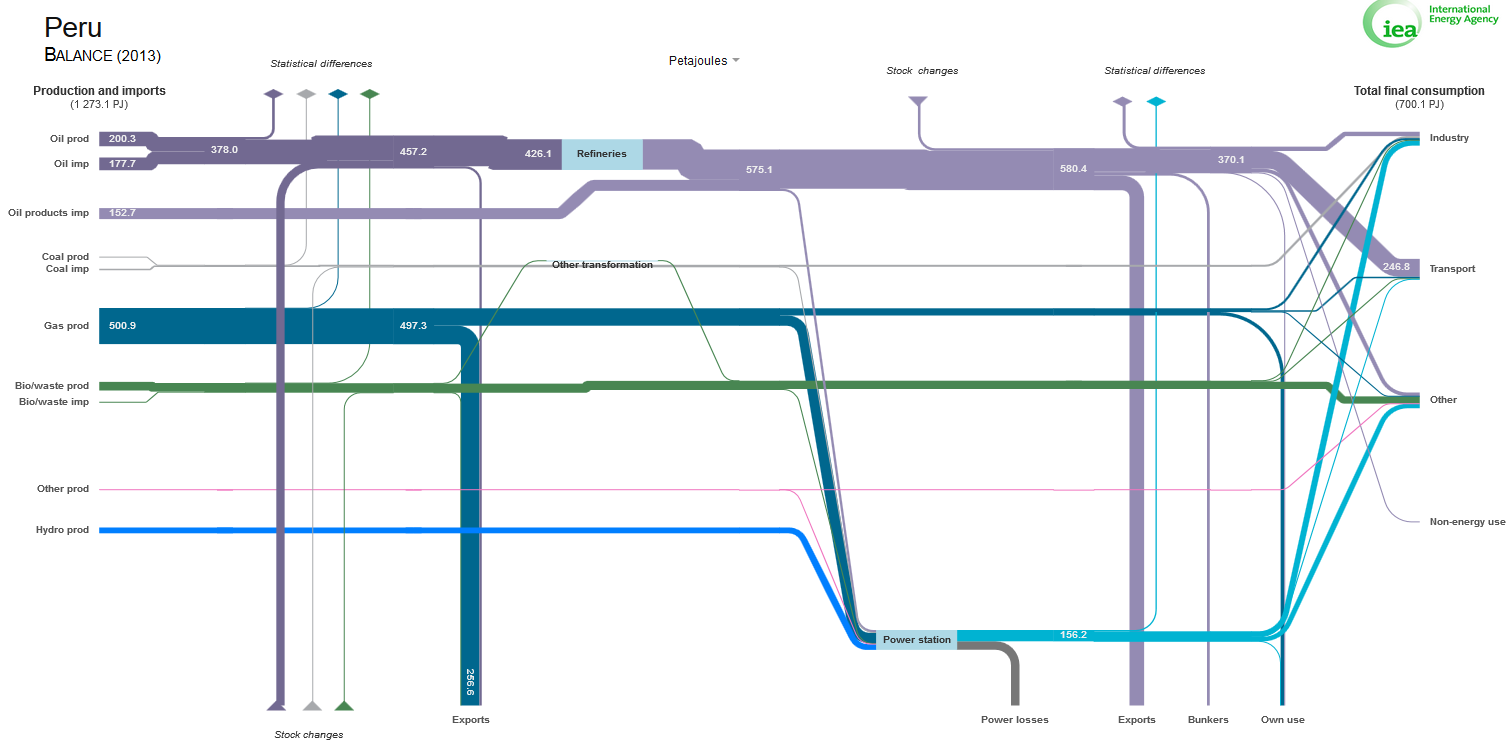
\includegraphics[width=0.80\linewidth]{imagenes/sankey_peru_2013}
%\caption[Diagrama de Sankey - Perú 2013]{Diagrama de Sankey - Perú 2013 (Fuente:\citep{iea_iea_2016} }
%\label{fig:sankeyperu2013}
%\end{figure}

Actualmente la generación de energía eléctrica eléctrica está "gasificada", considerando los bajos precios de gas provenientes  del lote 88. La participación de la energía eléctrica termoeléctrica (prácticamente producida toda con gas natural) tiene un porcentaje de participación similar a la energía hidroeléctrica y con una tendencia creciente [cita requerida de la memoria anual COES]. 
La actual construcción del gaseoducto al Sur y las nuevas plantas denominadas “Nodo energético” en Ilo y Mollendo, profundizarán e incrementarán el predominio del gas natural en la matriz energética nacional. Se espera así mismo incrementos en la participación de energías renovables (eólicas, solar y mini hidroeléctricas) pero  la participación de éstas  será minoritaria en el corto y mediano plazo \citep{coes_memoria_2016}.



%%%%%%%%%%%%%%%%%%%%%%%%%%%%%%%%%%%%%%%%%%%%%%%%%%%%%%%%%%%%%%%%%%%%%%%%%
%                           Objetivo                                    %
%%%%%%%%%%%%%%%%%%%%%%%%%%%%%%%%%%%%%%%%%%%%%%%%%%%%%%%%%%%%%%%%%%%%%%%%%

\section{Objetivo}

Este trabajo tiene por objetivo ...



%(Generales y específicos.)
\subsection{Objetivo General}

Cuantificar la energía producida por parques eólicos usando técnicas de Mecánica de Fluidos Computacional (CFD) y Modelos de Mesoescala de Predicción Numérica  Meteorológicos (NWP) utilizando el software OpenFOAM.

\subsection{Objetivos Específicos}

\begin{itemize}

\item Entender los fenómenos de mecánicas de fluidos involucrados en el funcionamiento de los parques eólicos
\item Modelar las características topográficas de la localización del Parque Eólico
\item Definir el tipo y modelo de turbinas eólicas que se analizarán.
\item Definir el arreglo general y ubicación de las turbinas eólicas
\item Definir el modelo simplificado  de intercambio de energía entre el flujo de viento y las turbinas eólicas. 
\item Definir las condiciones de frontera del volumen de control bajo estudio a partir de modelos numéricos climatológicos de meso-escala.
\item Elaboración de malla apropiada para los cálculos en el software OpenFOAM.
\item Determinar el tipo de flujo para usar el módulo apropiado del software OpenFOAM
\item Implementar el modelo utilizando el sofware OpenFOAM
\item Cuantificar la producción de energía para diferentes condiciones de operación y diferentes condiciones meteorológicas utilizando la similación numérica en OpenFOAM.
\item Comparar los resultados obtenidos con mediciones de campo existentes.
\item Evaluar los resultados obtenidos.
\end{itemize}


%%%%%%%%%%%%%%%%%%%%%%%%%%%%%%%%%%%%%%%%%%%%%%%%%%%%%%%%%%%%%%%%%%%%%%%%%
%                           Motivación y estado del arte                %
%%%%%%%%%%%%%%%%%%%%%%%%%%%%%%%%%%%%%%%%%%%%%%%%%%%%%%%%%%%%%%%%%%%%%%%%%
\section{Motivación}

El problema de calcular el viento sobre terrenos complejos ha recibido gran atención en los últimos años debido al incremento de la generación eléctrica con turbinas eólicas en diversas partes del mundo. La simulación numérica mediante la discretización de las ecuaciones de Navier-Stokes agiliza el desarrollo de los proyectos eólicos mediante una mejor estimación del recurso energético que hace viable a este tipo de proyectos.
\\
\\\subsection{Parque Eólicos}
En el caso de los Parque Eólicos, la producción de energía eléctrica depende de las características técnicas de los aerogeneradores las cuales son informadas por los fabricantes y por la disponibilidad del recurso eólico, que requiere de mediciones de largo plazo, \footnote{En las referencias  \citep{wbank_guidelines_2014}, \citep{sanz_state---art_2010} y \citep{bailey_wind_1997} se recomiendan tener un año de mediciones como mínimo aunque tres o cinco años son preferidos}. Estas mediciones se toman con un período de 10 minutos que incluyen velocidad y dirección del viento a diversas alturas entre 60 m y 100 m utilizando  sensores instalados en torres de medición instalada en el campo. 

Las mediciones de largo plazo tiene como objetivo de capturar las variaciones de largo plazo y reducir la incertidumbre de la medición. Dependiendo de la extensión del área y la complejidad de la topografía en la que estará emplazado el parque eólico pueden requerirse varias torres de medición que permitan cuantificar el recurso eólico en una localización específica, considerando que las torres registran medidas de velocidad y dirección del viento en un solo punto geográfico.

\subsection{Modelos Numéricos y Computacionales}

En la referencia \citep{wbank_guidelines_2014} se recomienda la realización de análisis basados en Mecánica de Fluidos Computacinal  (CFD) cuando otras técnicas simplificadas no permitan obtener resultados satisfactorios de extrapolación de las mediciones, esto suele ocurrir en casos con terreno complejos e inestabilidades que carecen de homogeneiodad del flujo como es asumido por las técnicas de medición de campo \citep{sanz_state---art_2010}.

Con la finalidad de mejorar la cuantificación de la energía producida por los parques eólicos se han propuestos diversas metodologías que combinan la Técnicas de Mecánica de Fluidos Computacional (CFD) y Modelos de Mesoescala de Predicción Numérica  Meteorológicos (NWP). 

Los modelos NWP del nivel de mesoescala permiten establecer condiciones de frontera de temperatura, presión y velocidad de viento para realizar cálculos locales en áreas algunas decenas de kilómetros cuadrados. 

Los modelos de CFD deben permitir retener la no linealidad de las ecuaciones de Navier Stokes tomando en cuenta el balance de momento los fenómenos de turbulencia adaptados a los flujos atmosféricos \citep{sanz_state---art_2010}. 


\subsection{Modelos CFD y NWP utilizados en la cuantificacion de Recursos de Parques Eólicos}

Las Mecánica  de Fluidos Computacional (CFD) (acotar a un tipo de técnica de CFD) y los Modelos Numéricos de Predicción Meteorológica requieren conocimientos extensos de Métodos Numéricos, lenguajes de programación, Mecánica de Fluidos, entre otros que no se estudian en los Planes de Estudio de Pre-grado de ingeniería, por lo cual constituye un tema apropiado para ser propuesto como tesis de maestría.

En \citep{beaucage_more_????} se indica que el modelo ampliamente aceptado de predecir la variación espacial de la velocidad promedio del viento es un modelo linealizado de flujo de viento\footnote{Los softwares para producir mapas de viento utilizan ampliamente este tipo de técnicas de bajo costo computacional}, considerando a las técnicas basadas en CFD como la siguiente generación para aplicaciones de energía. 

Los modelos numéricos acoplados con motores de calculo meteorológicos y de predicción del tiempo permiten una mayor sofisticación del cálculo a la vez que incrementan los requerimientos computaciones de las simulaciones, aunque este incremento computacional puede ser soportado por los computadoras disponibles hoy en día, como se observa en \citep*{zajaczkowski_preliminary_2011}. 

Estos modelos sofisticados han sido investigados tanto por instituciones como NREL, Universidad de Chalmers y otras así como soluciones comerciales propuestas por compañías consultoras como AWS. 

NREL (National Renewable Energy Laboratory) desarrolló un software prototípico "SOWFA" (Simulator fOr Wind Farm Application) que utiliza el software OpenFOAM acoplado con un modelo LES (Large Eddy Simulation) o RANS (Reynolds Average Navier-Stokes) \citep{stull_introduction_2012}. 

AWS ha investigado el desempeño de cuatro modelos numéricos (Jackson-Hunt, RANS CFD, NWP-Mass Consistent y NWP-LES) obteniendo desempeños que varían grandemente de sitio a sitio y considerando promisorio el modelo NWP-LES \cite{brower_evaluation_2013}.

\cite{bengtsson_turbulence_????} ha comparado modelos lineas, modelos CFD y modelos NWT, obteniendo mejores resultados con el método CFD.

\subsection{El software OpenFOAM}

OpenFOAM (acrónimo de ``Open source Field Operation And Manipulation") es una herramienta de cálculo programada en el lenguaje C++ orientada al desarrollo de motores de cálculo especializados, utilidades de pre y pos-procesamiento para la solución de problemas de mecánica continua.

OpenFOAM posee librerías  para la resolución de problemas de Mecánica de Fluidos Computacional (CFD). El código es libre y fuente abierta por lo que puede ser analizado y modificado en sus detalles \citep*{wikipedia_openfoam_2016}.




%%%%%%%%%%%%%%%%%%%%%%%%%%%%%%%%%%%%%%%%%%%%%%%%%%%%%%%%%%%%%%%%%%%%%%%%%
%                   Planteamiento del problema                          %
%%%%%%%%%%%%%%%%%%%%%%%%%%%%%%%%%%%%%%%%%%%%%%%%%%%%%%%%%%%%%%%%%%%%%%%%%

\section{Planteamiento del problema}


La cuantificación de la energía requiere mediciones de largo plazo de la velocidad y dirección del viento que permitan cuantificar el recurso eólico disponible en el emplazamiento del parque eólico. Las mediciones de campo se llevan a cabo mediante anemómetros y veletas localizados a diferentes alturas en las torres de medición. Con la información obtenida de estos sensores se estima la energía disponible en una localización específica a lo largo de la vida útil del parque eólico. 

Dependiendo de la extensión del emplazamiento y de la complejidad de la topografía del terreno pueden requerirse varias torres de medición para obtener una cuantificación confiable del recurso eólico. 

Las metodologías basadas únicamente en mediciones de campo tienen la desventaja de tomar en cuenta de manera muy pobre el impacto de la topografía y las variaciones locales del viento. Esto es así debido a la naturaleza discreta de la medición (una torre registra datos de un solo punto), a las dificultades prácticas de instalar una gran cantidad de torres de medición y a los errores inherentes a la extrapolación de la data medida en una área geográfica extensa.

La predicción de la energía producida por futuros Parques Eólicos puede mejorarse usando modelos de Mecánica de Fluidos Computacional (CFD) que retengan las características no lineales de las ecuaciones de Navier-Stokes como el balance de momento y los fenómenos turbulentos. Este modelo toma como condiciones de frontera los resultados de Modelos de Mesoescala de Predicción Numérica  Meteorológicos (NWP) correspondientes en un lugar y sitio específico donde está o estará localizado el Parque Eólico. 


%%%%%%%%%%%%%%%%%%%%%%%%%%%%%%%%%%%%%%%%%%%%%%%%%%%%%%%%%%%%%%%%%%%%%%%%%
%                           Metodología                                 %
%%%%%%%%%%%%%%%%%%%%%%%%%%%%%%%%%%%%%%%%%%%%%%%%%%%%%%%%%%%%%%%%%%%%%%%%%
\section{Metodología}

Se tiene un objetivo principal, y para llegar a \'el %otra forma de poenr acentos


así las ecuaciones de promedios de Reynold (RANS) y la caracterización de la  turbulencia mediante modelos de transporte de la energía cinética turbulenta y el ratio de disipación de esta energía (modelo $\kappa$-$\epsilon$ ) en estado estable han sido usados en el presente trabajo. Así mismo, la interacción entre el flujo turbulento del aire, los terrenos con topografía compleja y la capa límite atmosférica son analizadas, adicionalmente en estado dinámico utilizando el método de lattice-Boltzman (LBM).
\\
\\
\hspace*{1em}Se presenta una metodología para calcular la velocidad de viento, intensidad de turbulencia y otras magnitudes relevantes en las áreas extensas sobre la que se construyen parques eólicos. El calculo incluye valores a diferentes altitudes; así como, la interacción con las turbinas eólicas de modos que incluyen las pérdidas por estelas. Se utilizan los métodos RANS $\kappa$-$\epsilon$ (usando el código OpenFoam) y Lattice-Boltzman (usando el código OpenLB). Los resultados son validados mediante la resolución de problemas canónicos y comparaciones con valores medidos en el campo obteniendo resultados consistentes.

%Planteamiento de las ecuaciones:	5
%Discretización de las ecuaciones.	7
%Elaboración del mallado decalado (staggered grid).	8

\begin{itemize}
	\item Se propone una implementación de la cuantificación del Recurso Eólico de un parque  utilizando un enfoque físico (enfoque determinista) en oposición a un enfoque estadístico \citep*{wang_review_2011}.

Este método físico estará basado predicción de las condiciones de la baja atmósfera o predicción meteorológica  (NWP) usando los datos como temperatura, presión, rugosidad de la superficie y obtaculos.

\item En general, la velocidad de viento es obtenida de los Sistemas que ofrecen información sobre condiciones meteorológicas \citep*{wang_review_2011}. 

Pará el Perú esta información están disponible previsiones numéricas dos veces al día con el modelo regional Eta para los dominios: Perú (22 Km) y Sudamérica (32 Km). Las condiciones iniciales y de frontera son obtenidas del modelo Global Forecast System (GFS) \citep{senamhi_servicio_????}. 

\item La información topográfica es convertida a un formato utilizable en OpenFOAM desde data obtenida y procesadas en sistemas de información geográfica como GRASS o QGIS, como se describe en \citep{hardin_how_2013}.

\item Los modelos son resueltos en OpenFOAM y los resultados son analizados y evaluados.
\end{itemize}

En la figura \ref{fig:metodo} se observa la etapas que se seguirán para realizar los cálculos propuestos. ESte muestra un ejemplo tomado de \citep{stull_introduction_2012} en el cual requirió un tiempo de procesamiento de 21 horas para 750 segundos de simulación corriendo en un arreglo de 64 procesadores.

\begin{figure}[h!]
\centering
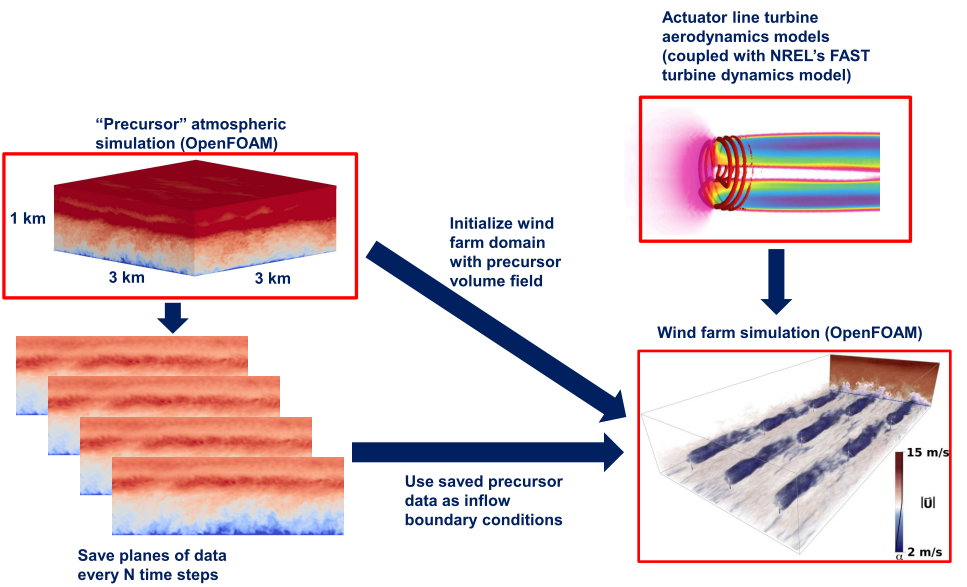
\includegraphics[width=0.8\linewidth]{imagenes/metodo}
\caption[Metodo de Cálculo]{Método de Cálculo (Fuente: \citep{stull_introduction_2012})}{}
\label{fig:metodo}
\end{figure}



%%%%%%%%%%%%%%%%%%%%%%%%%%%%%%%%%%%%%%%%%%%%%%%%%%%%%%%%%%%%%%%%%%%%%%%%%
%                         Contribuciones                                %
%%%%%%%%%%%%%%%%%%%%%%%%%%%%%%%%%%%%%%%%%%%%%%%%%%%%%%%%%%%%%%%%%%%%%%%%%

\section{Contribuciones}

La principal contribución de este trabajo es 
\blindtext
%%%%%%%%%%%%%%%%%%%%%%%%%%%%%%%%%%%%%%%%%%%%%%%%%%%%%%%%%%%%%%%%%%%%%%%%%
%                           Estructura de la tesis                      %
%%%%%%%%%%%%%%%%%%%%%%%%%%%%%%%%%%%%%%%%%%%%%%%%%%%%%%%%%%%%%%%%%%%%%%%%%

\section{Estructura de la tesis}

Este trabajo está dividido en XX capítulos. Al principio se encuentra 
\\\\
Finalmente se encuentra la parte de 